\documentclass{tcvg}
\usepackage{mathptmx}
\usepackage{graphicx}
\usepackage{eso-pic,calc}
\usepackage{color}
\usepackage{url}
\usepackage[pdftex]{hyperref}
\usepackage[compact]{titlesec}
\usepackage{framed}
\usepackage{watermark}

\titlespacing*{\section}{0pt}{11pt}{3pt}


% shorthand for href email addresses...
\newcommand{\email}[1] {\href{mailto:#1}{#1}}

\definecolor{off-white}{rgb}{0.2,0.2,0.2}
\definecolor{shadecolor}{rgb}{0.98,0.98,0.98}
\definecolor{darkgreen}{rgb}{0,0.5,0}
\definecolor{darkblue}{rgb}{0,0,0.5}
\definecolor{darkred}{rgb}{0.5,0,0}

\hypersetup{
    unicode=false,          % non-Latin characters in Acrobat’s bookmarks
    pdftoolbar=true,        % show Acrobat’s toolbar?
    pdfmenubar=true,        % show Acrobat’s menu?
    pdffitwindow=false,     % window fit to page when opened
    pdfstartview={FitH},    % fits the width of the page to the window
    pdftitle={Programming Models for Extreme-Scale Visualization and Data Analysis},
    colorlinks=true,        % false: boxed links; true: colored links
    linkcolor=darkblue,     % color of internal links
    citecolor=darkgreen,    % color of links to bibliography
    filecolor=magenta,      % color of file links
    urlcolor=darkblue       % color of external links
}

\title{Programming Models for Extreme-Scale\\ 
         Visualization \& Data Analysis}


\newcommand{\backgroundpic}[1] {
	\ClearShipoutPicture
	\AddToShipoutPicture{
		\put(0,0) {
			\parbox[b][\paperheight]{\paperwidth}{
				\vfill
				\centering
				\includegraphics[width=\paperwidth,height=\paperheight,keepaspectratio]{#1}
				\vfill
			}
		}
	}
}

\begin{document}
	
  \backgroundpic{figures/bg-front.pdf}

  \maketitle 

  %\section*{Introduction}

   Over the past twenty years the Department of Energy (DOE) has firmly 
   established the fundamental role that high-performance computing 
   plays in a wide range of scientific disciplines.  Today this success
   faces several critical challenges as rapid changes in the design of 
   computer architectures impacts our abilities to effectively program  
   future systems and ever-increasing amounts of data continue to 
   overwhelm our capabilities to explore, analyze, hypothesize, and 
   thereby successfully interpret the underlying phenomena. While the 
   full range of topics covered by these challenges are often viewed 
   individually, we believe it is critical that they be considered in 
   concert with the goal of improving the rate of scientific innovation
   and discovery.  This will require an \emph{end-to-end} solution that 
   begins with the details of the underlying computer hardware and ends 
   with a set of powerful abstractions that reduce the complexity of 
   programming not only the scientific application itself but also the 
   supporting data analysis operations. 

  \section*{Science-Centric Strategy}

   The overarching goal of our effort is to provide scientists with an 
   approach to software development that promotes the full integration of 
   computation, data analysis, and visualization as \emph{first-class} 
   constructs within a programming language.  This not only serves to 
   improve productivity, but also provides a focused interface for 
   dealing with the specific needs of the scientific community.  This 
   methodology is commonly referred to as a \emph{domain-specific} 
   approach to programming and it provides several attractive properties
   for dealing with the emerging challenges of extreme-scale computing.
   This allows us to tailor an approach geared to the needs of the 
   community that in particular address the challenges of rapidly changing
   computer hardware and data-centric operations. 

   Increasing limitations in the infrastructure for moving data within a 
   large-scale computer, relative to the scale of the data the system is 
   capable of generating, will force scientists away from a model of 
   post-processing data, stored in secondary or tertiary memory,
   towards one based on \emph{in situ} processing.  Given that the movement of 
   data is a significant portion of the energy consumption and directly 
   impacts performance, this \emph{in situ} mode of operation will require 
   a strongly coupled coordination between the science-focused and 
   data-centric components of an application. 
    
   Increasing limitations 
   in the I/O infrastructures of large-scale supercomputers, relative to the 
   scale of the data the systems will generate, are likely to force scientists 
   away from the post-processing of data towards a model based on in situ 
   processing. 


    This is achieved by designing and implementing a
   \emph{domain-specific language} (DSL~\cite{Fowler:DSL:2010}) called
   Scout that incorporates these features into a supporting
   set of high-level abstractions.  Figure~\ref{fig:spasm} presents an
   example of an image produced using this approach. In this case,  
   particular elements from a materials data set are selected, used to derive associated
   features and values of interest, and then mapped to a given visual
   representation.  In this way, the approach to programming becomes
   much more representative and descriptive of the overall workflow.
   This also enables the DSL compiler to better understand the full
   context of the supporting computations and leverage that information
   to improve both optimization and code generation.  This is in direct 
   comparison to the common approach of using disparate software components 
   that are typically integrated at a coarse-grained level.  As is typical with 
   most DSLs, our supporting set of abstractions, syntax, and semantics 
   are designed to provide application scientists with a more expressive 
   and natural mapping for computations while shielding them from the nuances
   of the underlying low-level software and hardware architectures.

 	\begin{figure}[b!]
	  \centering
	  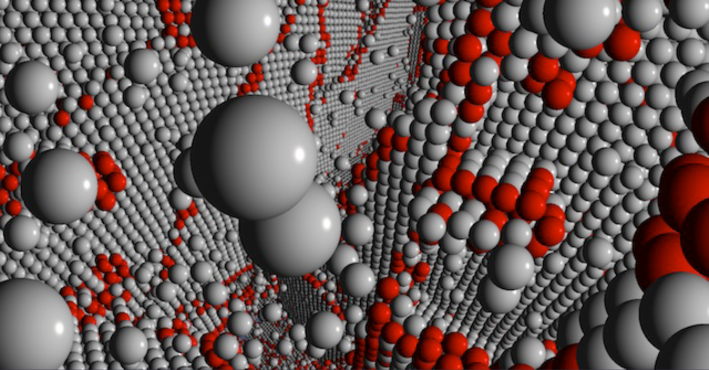
\includegraphics[width=3.25in]{figures/spasm.png}
	  \caption{Programmatically selected atoms in a copper block
         that has been subjected to a shock.  The gray atoms 
         show stacking faults and red represents non-close-packed 
         atoms.  Our approach allows scientists to program accelerator-based
         architectures at a high-level of abstraction where these images can 
         be generated at 30-60 frames per second for tens to hundreds of 
         millions of atoms.}
	  \label{fig:spasm}
	\end{figure}

  \section*{Language Design}

    The fundamental abstraction within Scout is that of a computational mesh
    while the language introduces explicit mesh declarations, instantiations,
    and parallel computation over the various components of the mesh (e.g. cells, 
    vertices, edges).  This abstraction and a restricted set of operations are
    also used within the Liszt DSL developed at Stanford 
    University~\cite{DeVito:2011:LDS}.  In addition Scout
    adds features allowing the programmer to control details of how  
    mesh components are visualized based on field values stored within the mesh, and/or 
    derived values computed during the visualization process. We are actively 
    exploring how best to provide programmatic interfaces for supporting multiple 
    visual mappings (e.g. graphs, glyphs, etc.). Unlike C and C++, the underlying 
    data layout details for mesh constructs are not available to the developer 
    and are instead determined by the compiler. The source listing in 
    Figure~\ref{fig:source} provides a brief overview of the mesh constructs 
    from the Scout language. 
     
	\begin{figure}[b!]
		\centering
		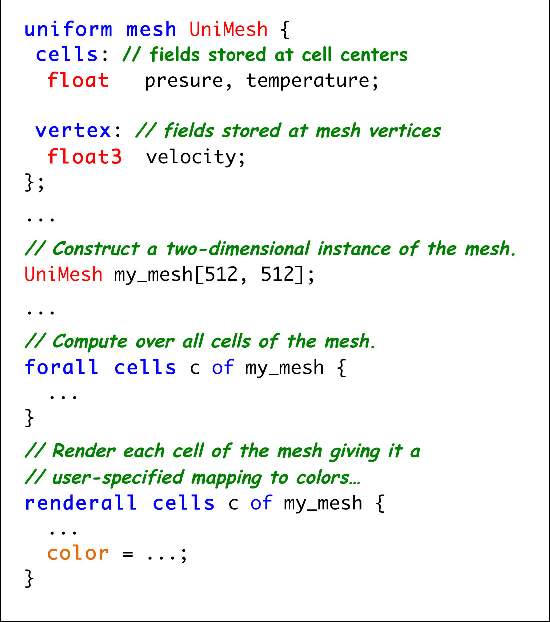
\includegraphics[width=3.00in]{figures/source-fig-v2.pdf}
		\caption{An example of Scout's mesh types and supporting language constructs.}
	\label{fig:source}
   \end{figure}

 \begin{figure*}[ht]
		\centering
		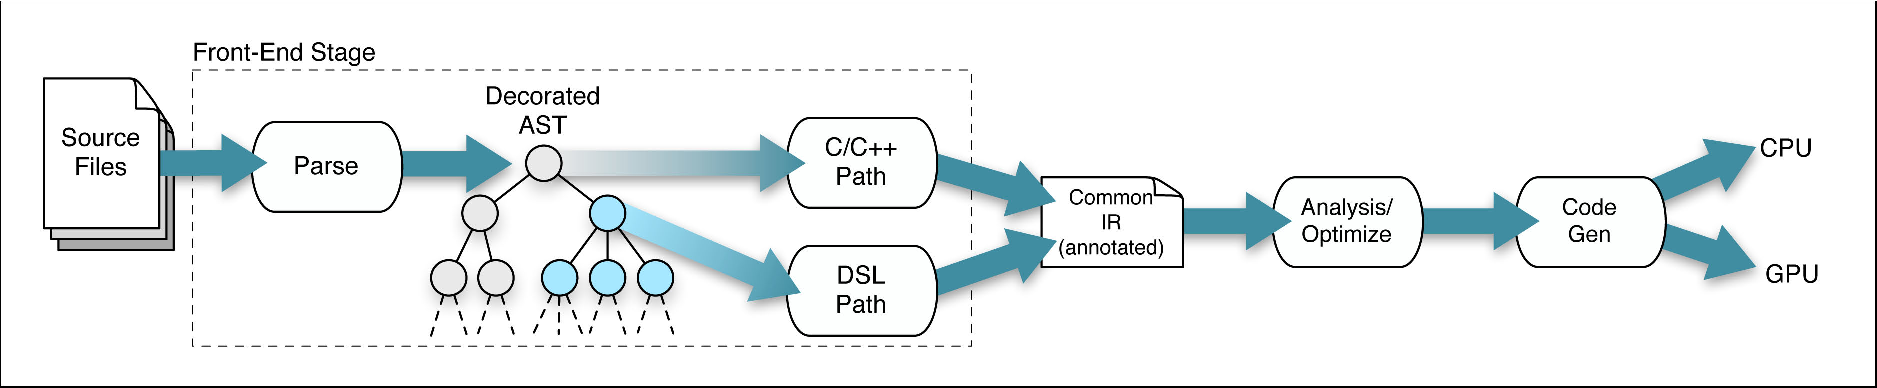
\includegraphics[width=7in]{figures/toolchain-v2.pdf}
		\caption{The Scout compiler toolchain leverages an extended
          C/C++ infrastructure allowing DSL and general-purpose 
          constructs to co-exist within a single program.  This 
          approach allows the majority of the traditional compiler 
          toolchain to remain intact, leveraging the broader efforts 
          taking place within the Clang and LLVM communities.  This
          has noticeably increased our flexibility to explore 
          the power of a full compiler toolchain and has 
          reduced the overall costs of development activities.}
	\label{fig:toolchain}
    \end{figure*}

  \section*{Compiler Toolchain}

    Our strategy for implementing Scout is to extend C/C++ to
    support the new set of abstractions and domain-specific constructs. 
    This approach reduces the learning curve of an entirely 
    new language, supports a smoother transition to the adoption of new
    methods of programming, and decreases some of the complexity of interoperating
    with legacy codes.  We have based our work on the open-source
    Clang and LLVM Compiler Infrastructure~\cite{Clang:2012,LLVM:2012}.  
    Furthermore, this avoids the necessity of implementing an entire 
    compiler toolchain -- instead focusing on the details of supporting 
    the domain-specific features and the associated runtime components.
    Finally, the adoption of a full compiler infrastructure provides  
    the flexibility to maintain and leverage domain-centric knowledge throughout the
    entire compilation process -- something
    difficult to achieve when using a \emph{source-to-source} approach. 
    Figure~\ref{fig:toolchain} presents a
    high-level view of the modified compiler toolchain.  Note that the
    DSL portions of the code are recognized and processed separately 
    based on the abstract syntax tree (AST) representation of the program.
    Next both the C/C++ and DSL code are lowered to LLVM's common 
    intermediate representation (IR); a key difference being that the IR
    from the DSL side still retains domain-specific annotations. At this 
    stage, the IR can pass through both a common set of analysis and 
    optimization passes as well as tailored, domain-centric passes. Using 
    this approach we can take a single Scout program and target sections 
    of a single program to a combination of sequential, multi-core CPU, 
    and GPU code generation targets.

  \backgroundpic{figures/bg-back.pdf}

    Initial results of this approach have shown distinct advantages to
    programmatically expressing the mappings from data to visual results.
    In particular, the expressiveness of a programming language in 
    comparison to the traditional approach of user interface-driven tools, 
    has shown promise.  Along these lines, we are actively exploring the 
    use of Scout toolchain within a mixed-language environment for 
    supporting the \emph{in situ} visualization of results within modern
    application codes.  These experiments are designed to help us not 
    only evaluate the overall approach, but to also better understand how
    the requirements and needs across different scientific disciplines
    impact the design and underlying implementation of the domain-specific
    language.  

  \bibliographystyle{plain}
  \bibliography{flyer}

  %\vspace{0.25in}

  \begin{snugshade}
	\vspace{-0.1in}
    \begin{tabbing}
	  ~~ \= ~~ \= ~~ \= ~~ \=\\
      \emph{For more information contact:}\\
	  \\
      \noindent 
      \> \textbf{Principal Investigator:}\\
	  \>\> Patrick McCormick\\
	  \>\> Los Alamos National Laboratory\\
	  \>\> Phone: 505-665-0201\\
	  \>\> Email: \email{pat@lanl.gov}\\
      \\
	 \> \textbf{Program Manager:}\\
	  \>\> Dr. Lucy Nowell\\
	  \>\> Advanced Scientific Computing Research Office\\
	  \>\> Phone: 301-903-3191\\
	  \>\> Email: \email{lucy.nowell@science.doe.gov}
	\end{tabbing}
  \end{snugshade}  

\end{document}
